\documentclass[a4paper,fleqn,12pt]{article}
%\usepackage[T1]{fontenc}
\usepackage[brazilian]{babel}
%\usepackage[utf8]{inputenc}
\usepackage[left=2.5cm,right=2.5cm,top=3cm,bottom=2.5cm]{geometry}
\usepackage{mathtools}
%\usepackage{amsthm}
%\usepackage{amsmath}
%\usepackage{nccmath}
%\usepackage{amssymb}
\usepackage{amsfonts}
\usepackage{physics}
%\usepackage{dsfont}
%\usepackage{mathrsfs}

\usepackage{titling}
\usepackage{indentfirst}

\usepackage{bm}
\usepackage[dvipsnames]{xcolor}
\usepackage{cancel}

\usepackage{xurl}
\usepackage[colorlinks=true]{hyperref}

% code
\definecolor{bg}{rgb}{0.90,0.90,0.90}
\usepackage{minted}


%\usepackage{float}
%\usepackage{graphicx}
%\usepackage{tikz}
%\usepackage{caption}
%\usepackage{subcaption}

%%%%%%%%%%%%%%%%%%%%%%%%%%%%%%%%%%%%%%%%%%%%%%%%%%%

\newcommand{\eps}{\epsilon}
\newcommand{\vphi}{\varphi}
\newcommand{\cte}{\text{cte}}

\newcommand{\N}{\mathbb{N}}
\newcommand{\Z}{\mathbb{Z}}
\newcommand{\Q}{\mathbb{Q}}
\newcommand{\R}{\mathbb{R}}
%\newcommand{\C}{\mathbb{C}}
\renewcommand{\H}{\hat{H}}
\newcommand{\intR}{\int_{-\infty}^{\infty}}

\newcommand{\0}{\vb{0}}
\newcommand{\1}{\mathds{1}}
\newcommand{\E}{\vb{E}}
\newcommand{\B}{\vb{B}}
\renewcommand{\v}{\vb{v}}
\renewcommand{\r}{\vb{r}}
\renewcommand{\k}{\vb{k}}
\newcommand{\p}{\vb{p}}
\newcommand{\q}{\vb{q}}
\newcommand{\F}{\vb{F}}

\renewcommand{\a}{\hat{a}}
\renewcommand{\b}{\hat{b}}
\renewcommand{\c}{\hat{c}}
\newcommand{\nn}{\hat{n}}

\newcommand{\gf}[2]{\ev{\ev{#1 : #2}}}
\newcommand{\zub}[2]{\ev{\comm{#1}{#2}_\mp}}

\newcommand{\s}[1]{\mathcal{#1}}
%\newcommand{\prodint}[2]{\left\langle #1 , #2 \right\rangle}
\newcommand{\cc}[1]{\overline{#1}}
\newcommand{\Eval}[3]{\eval{\left( #1 \right)}_{#2}^{#3}}

\newcommand{\unit}[1]{\; \mathrm{#1}}

\newcommand{\n}{\medskip}
\newcommand{\e}{\quad \mathrm{e} \quad}
\newcommand{\ou}{\quad \mathrm{ou} \quad}
\newcommand{\virg}{\, , \;}
\newcommand{\ptodo}{\forall \,}
\renewcommand{\implies}{\; \Rightarrow \;}
%\newcommand{\eqname}[1]{\tag*{#1}} % Tag equation with name

% math %
\renewcommand{\erf}[1]{\text{erf}\left(#1\right)}
\newcommand{\floor}[1]{\left\lfloor #1 \right\rfloor}
\newcommand{\ceil}[1]{\left\lceil #1 \right\rceil}

\setlength{\droptitle}{-6em}


\title{\Huge{\textbf{P1 - Statistical Learning}}}
\author{Mateus Marques}

\begin{document}

\maketitle

\section{Intro}

\subsection{Conceitos}

\begin{itemize}
\item Missing data: é quando uma variável não é observada.
\item Missing data at random: algumas variáveis não são observadas em alguns dados de maneira aleatória. Missing data due to systematic reason: existe alguma razão sistemática em que variáveis não são observadas.
\item Data prep: é o processo de manipular os dados brutos para que eles estejam prontos para serem analisados. Tarefas usuais são:
\begin{itemize}
\item integração de dados (colocá-los no mesmo formato, unidades etc.).
\item entender os dados (fazer plots, histogramas etc. para ter uma ideia do dataset).
\item discretizar, normalizar os dados.
\item remover outliers (dados muito fora do resto).
\item fazer algo sobre missing data.
\item feature selection.
\end{itemize}
\item Handling missing data:
\begin{itemize}
\item remover linhas ou colunas.
\item imputar a média, mediana ou moda.
\item regressão de outras variáveis.
\item predição, estimação, interpolação.
\end{itemize}
\item Feature: as variáveis que são observadas, correspondem ao $X_1, X_2, \ldots, X_n$.
\item Label (rótulo): valores da variáveis \textit{de classe (target)} $Y$ (a que se tem interesse).
\item Supervised learning: quando não temos missing labels (dados do $Y$ estão todos presentes).
\item Unsupervised learning: quando todo rótulo $Y$ está faltando.
\item Semi-supervised learning: alguns labels estão faltando (caso geral).
\item Classifier: é uma função $g(X_1, \ldots, X_n)$ que produz labels $\hat{Y}$ em função dos features $X_1, \ldots, X_n$. Produzir uma função $g$ usando os dados é chamado \textit{treinamento do classificador}.
\item Classification: é quando $Y$ tem valores discretos.
\item Regression: é quando $Y$ tem valores contínuos.
\item Training dataset: conjunto de dados utilizados para treinar o classificador (produzi-lo).
\item Testing dataset: conjunto de dados utilizados para testar o classificador. Por exemplo estimando a taxa de erro empiricamente.
\item Error rate: taxa de erro é a probabilidade do classificador errar $e_g = P(Y \neq g(\vb{X}))$.
\item Empirical error rate: taxa de erro empírica é a proporção que ele errou nos dados de teste $\hat{e}_g = \frac{\text{número de vezes que }Y \neq g(X)}{\text{número total de tentativas}}$.
\item Overfitting: o classificador é muito bom nos dados de teste, mas ele falha para outros dados. Um exemplo é o $1NN$. Nos dados de teste a taxa de erro é sempre zero, mas nos de teste pode ser alta. Outro exemplo é quando o modelo do classificador é muito complexo para o fenômeno, tipo quando se tenta fitar um polinômino de grau 1000 num fenômeno essencialmente linear.
\item Underfitting: o classificador treinou pouco demais, o modelo dele é muito simples para conseguir capturar a complexidade do fenômeno. Por exemplo tentar fitar uma reta em um fenômeno altamente não-linear.
\item Cross-validation: quando não se tem dados suficiente para criar um \textit{holdout} (separar uma parte dos dados para teste, tipo uns $30\%$) para testar, então usamos validação cruzada. A ideia é separar uma fração dos dados totais para testar, e ir repetindo sobre toda a base de dados.
\begin{figure}[H]
\centering
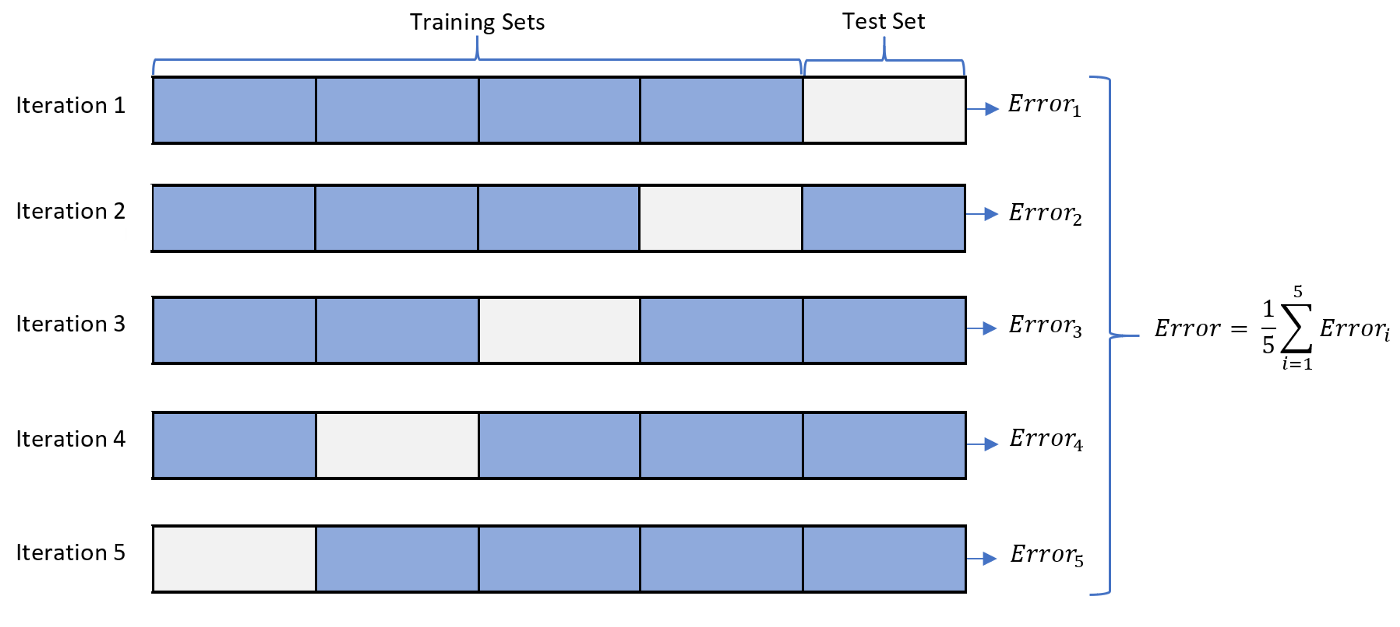
\includegraphics[width=0.8\textwidth]{fig/crossval.png}
\caption{Diagrama de validação cruzada.}
\label{fig:crossval}
\end{figure}
\item Leave-one-out validation: (é o extremo da validação cruzada) se você tem $N$ linhas de dados, a ideia é fazer validação cruzada com $N$ iterações, sempre deixando um dado para teste de fora em cada separação e depois computando o erro médio sobre as $N$ etapas.
\item Validation dataset: parte dos dados que não participam do treino e são utilizados para dar estimativas para a eficiência do classificador e tunar os hiperparâmetros. É diferente do testing dataset, pois o testing dataset é utilizado depois dos hiperparâmetros já terem sido tunados e ele serve para dar uma estimativa imparcial da qualidade do classificador escolhido (através da validação).
\item Stratified cross-validation: validação cruzada, porém com uma divisão que respeita a proporção de labels para cada divisão.
\begin{figure}[H]
\centering
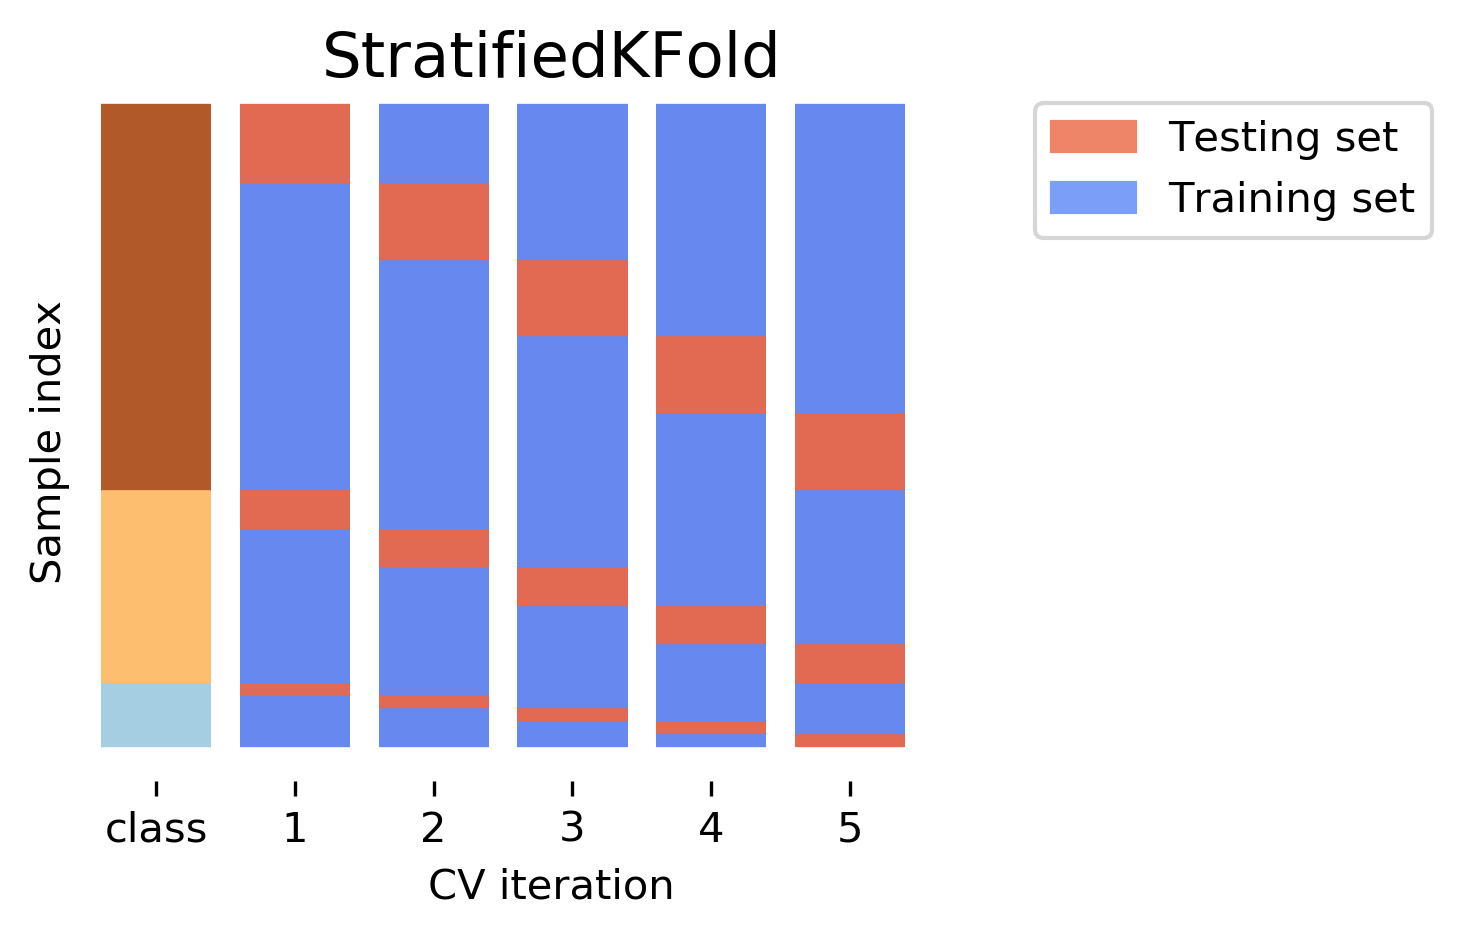
\includegraphics[width=0.8\textwidth]{fig/strcrossval.png}
\caption{Validação cruzada estratificada.}
\label{fig:strcrossval}
\end{figure}
\item Bayes classifier: o classificador ótimo, aquele em que dadas a probabilidade $P(Y = y | X=x)$, ele escolhe o $\hat{Y}=y$ tal que a probabilidade é a maior.
\item Bayes error: o menor erro que pode ser cometido por um classificador. É o erro que o classificador de Bayes comete.
\item Plug-in classifier: tentar estimar as probabilidades $P(Y=y | X=x)$ através de algum modelo, e então utilizar a fórmula do classificador de Bayes.
\item Nearest-neighbor classifier: classificar cada ponto de acordo com uma média entre $k$ vizinhos mais próximos dos dados de treino.
\item Teorema sobre kNN: seja $n$ o número de observações no training dataset. Se $k = k(n) \to \infty$ de maneira que $k(n)/n \to 0$, então $\lim_{n \to \infty} E[e_{g_n}] = e_{g^*}$. Ou seja, se pegarmos $k$ tendendo ao infinito mas de maneira que ele seja sempre superado pelo número de observações $n$, então a taxa de erro do $kNN$ tende para o menor erro possível (erro de Bayes).
\item Teorema sobre 1NN: temos para o 1NN que $\lim_{n\to\infty} E[e_{g_n}] \leq 2e_{g^*}$. Ou seja, o erro do 1NN para infinitos dados sempre será menor que duas vezes o erro de Bayes.
\end{itemize}

\subsection{Regression}

Assumimos que $Y = f(X) + \eps$, onde $\eps$ é um erro aleatório independente com média zero e variância $\sigma^2$. Nós queremos $\hat{Y} = \hat{f}(X)$ para alguma estimativa $\hat{f}$. A medida usual é minimizar o \textit{expected quadratic error} $E[(Y-\hat{Y})^2]$.

Se $\hat{f}$ for muito simples, então caímos em \textit{underfitting}. Se $\hat{f}$ for muito complexo caímos em \textit{overfitting}. Para isso, monitoramos o \textit{mean squared error} com respeito aos dados de TESTE
$$
\frac{1}{N} \sum_{i=1}^N \Big(y_i - \hat{f}(x_i)\Big)^2,
$$
que se trata de uma estimativa para $E[(Y-\hat{Y})^2]$.

Seja $D$ o training dataset. A partir de $D$, nós treinamos um classificador $\hat{Y} = \hat{f}(X, D)$. O erro quadrático esperado é
$$
E[(Y-\hat{Y})^2] = E\Big[E[(Y-\hat{Y})^2 | x]\Big].
$$
Temos então a seguinte decomposição
$$
E[(Y-\hat{Y})^2 | x] = E[(f + \eps - \hat{f} )^2 | x] = E\qty[\Big((f - E[\hat{f}|x]) + \eps + (E[\hat{f}|x] - \hat{f}) \Big)^2 | x] =
$$
$$
E[(f-E[\hat{f}|x])^2|x] + E[\eps^2|x] + E[(E[\hat{f}|x]-\hat{f})^2|x] \; +
$$
$$
2E[(f-E[\hat{f}|x]) \eps|x] + 2E[\eps (E[\hat{f}|x] - \hat{f})|x] +
2E[(f-E[\hat{f}|x]) (E[\hat{f}|x] - \hat{f})|x]
$$
Na expressão acima, cada um dos termos da segunda linha é igual a zero. Pois
\begin{itemize}
\item $f$ é ``constante'' com respeito a $E[\cdot | x]$ e a média de $\eps$ é nula $E[\eps | x] = 0$.
$$
2E[(f-E[\hat{f}|x]) \eps|x] = 2 (f-E[\hat{f}|x]) \cancelto{0}{E[\eps|x]} = 0
$$
\item A variável $\eps$ é independente de $\hat{f}$.
$$
2E[\eps (E[\hat{f}|x] - \hat{f})|x] = 2 \cancelto{0}{E[\eps|x] \, E[(E[\hat{f}|x] - \hat{f})|x]} = 0.
$$
\item $f$ é ``constante'' com respeito a $E[\cdot | x]$.
$$
2E[(f-E[\hat{f}|x]) (E[\hat{f}|x] - \hat{f})|x] = 2 (f-E[\hat{f}|x])
\cancelto{0}{E[(E[\hat{f}|x] - \hat{f})|x]} = 0
$$
\end{itemize}
Temos então
$$
E[(Y-\hat{Y})^2] = E\Big[E[(Y-\hat{Y})^2 | x]\Big] =
$$
$$
E\Big[E[\eps^2|x] + (f-E[\hat{f}|x])^2 + E\big[(E[\hat{f}|x]-\hat{f})^2|x\big]\Big]=
$$
$$
E[\eps^2] + E\Big[(f-E[\hat{f}|x])^2\Big] + E\Big[E\big[(E[\hat{f}|x]-\hat{f})^2|x\big]\Big] \implies
$$
$$
\boxed{E[(Y-\hat{Y})^2] = \sigma^2 + E[\text{bias}^2] + E[\text{variance of }\hat{f}],}
$$
where
$$
\text{bias} = f(x) - E[\hat{f}(x, D) | x],
$$
$$
\text{variance} = E\qty[\Big(\hat{f}-E[\hat{f}|x]\Big)^2\mid x] = E[\hat{f}(x, D)^2 | x] - E[\hat{f}(x, D) | x]^2.
$$

A ideia intuitiva é
\begin{itemize}
\item Um estimador simples geralmente tem vício alto, porém com pouca variância.
\item Um estimador complexo geralmente tem vício pequeno, porém variância alta.
\end{itemize}

\section{Evaluation}

\subsection{Confusion Matrix}

A matriz de confusão compara o rótulo de fato (actual label, true class) com o valor dito pelo classificador (predicted class). A primeira letra diz respeito se o actual label é igual ao que foi dito pelo classificador, T = True ou F = False. A segunda letra diz respeito ao valor dito pelo classificador, P = Positive ou N = Negative. Assim temos
$$
\begin{pmatrix}
\text{TP} & \text{FP} \\
\text{FN} & \text{TN}
\end{pmatrix},
$$
ou a Figura \ref{fig:confusion-matrix} abaixo.
\begin{figure}[H]
\centering
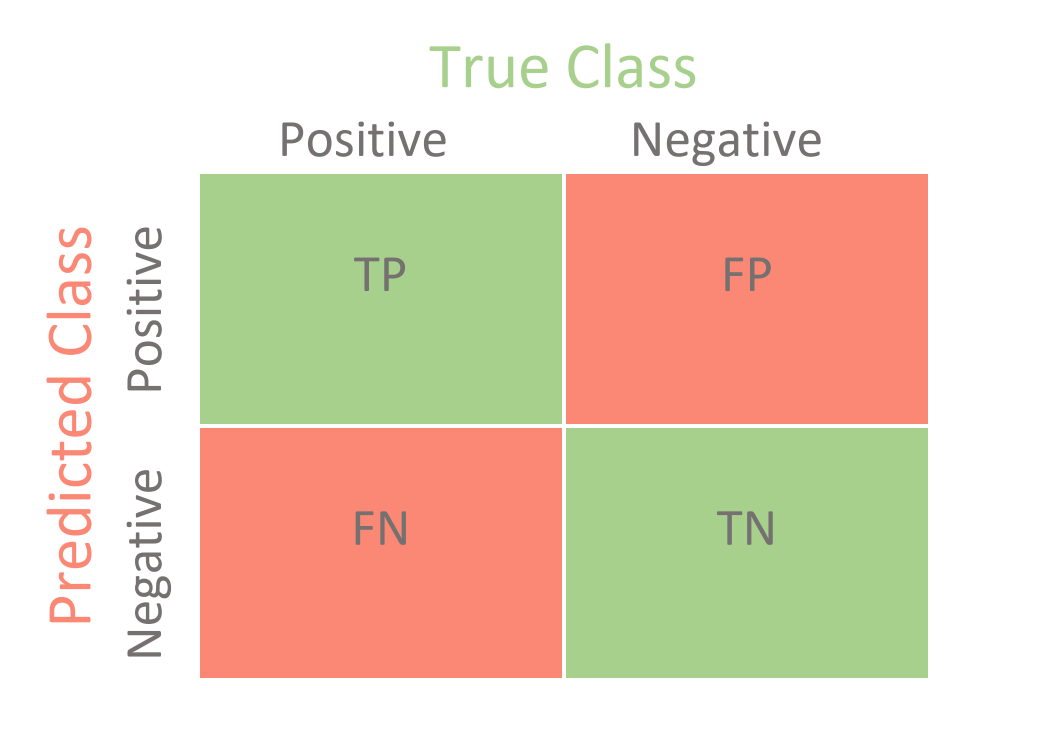
\includegraphics[width=0.5\textwidth]{fig/confusion-matrix.png}
\caption{Matriz de confusão.}
\label{fig:confusion-matrix}
\end{figure}

A acurácia é o quanto o classificador acertou (deu \texttt{True}) dentre tudo que ele falou. Ou seja
$$
\text{Accuracy} = \frac{\text{TP}+\text{TN}}{\text{TP}+\text{FP}+\text{FN}+\text{TN}}
= \frac{\text{true}}{\text{all}}.
$$
Alguns problemas com a acurácia são
\begin{itemize}
\item No caso de classes desbalanceadas, onde se tem muito mais certo label do que outro. Nesse caso, somente falando o label mais abundante você tem uma acurácia muito alta, porém um classificador burro.
\item Alguns erros são piores que outros. No caso da medicina, um falso negativo (não detectar doença existente) é muito pior que um falso positivo (detectar doença inexistente).
\end{itemize}

A precisão é quanto o classificador acerta quando se tem realmente o label. Ou seja
$$
p = \text{Precision} = \frac{\text{TP}}{\text{TP}+\text{FP}} = \frac{\text{true positive}}{\text{positive}} = \frac{\text{true positive}}{\text{get the label}}.
$$
Note que no caso de uma doença, um classificador tem alta precisão se ele conseguiu detectar uma fração grande de pessoas que tem doença dentre as que ele falou que tinha (quanto ele acertou sobre quanto ele falou).

A revocação (\textit{recall}) é a TP rate. Ou seja, TP dividido pela soma da coluna. Assim
$$
r = \text{Recall} = \frac{\text{TP}}{\text{TP} + \text{FN}} = \frac{\text{true positive}}{\text{have the label}}.
$$
A ideia da revocação é quanto a taxa que o classificador acerta dentre as pessoas que possuem o label. Isso é uma medida de quanto ele é cuidadoso com o label. Se ele tiver uma revocação alta, quer dizer que dentre as pessoas que tem o label, ele toma um certo cuidado em maximizar o acerto.

Todas as rates é ela mesmo dividida pela soma da coluna. Então, TN rate é $\frac{\text{TN}}{\text{TN} + \text{FP}}$.

Sendo $p$ a precisão e $r$ a revocação, $F_1$ é a média harmônica
$$
\frac{2}{F_1} = \frac{1}{p} + \frac{1}{r} \implies F_1 = \frac{2pr}{p+r}.
$$
Note que sempre $F_1 \leq \min(p, r)$.

\subsection{Curva ROCK}

Nós só definimos a curva ROC para classificadores que sejam da seguinte maneira:
\begin{itemize}
\item Para cada observação $x$ ele calcula um número $h(x)$.
\item Então ele classifica $\hat{Y} = 1$ se $h(x) > \alpha$ e $\hat{Y} = 0$ caso contŕario.
\end{itemize}
A curva ROC (Receiver Operating Characteristic) captura a influêncida do $\alpha$.

Para classificadores plug-ins que tentam minimizar o custo $c(\hat{Y}, Y)$:
\begin{figure}[H]
\centering
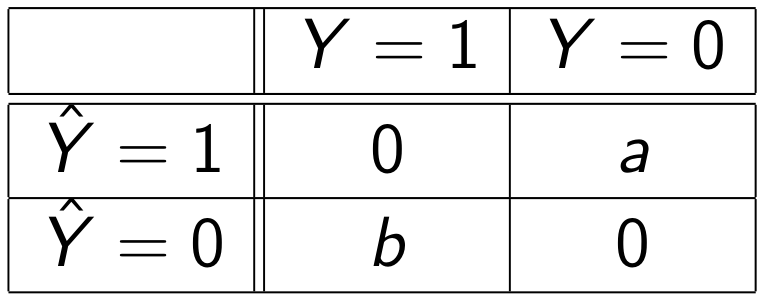
\includegraphics[width=0.6\textwidth]{fig/cost.png}
\caption{Custo com pesos $a$ e $b$.}
\label{fig:cost}
\end{figure}
$$
E[c(\hat{Y}, Y)] = \sum_x P(X = x)
\begin{cases}
b \, P(Y=1|x) \text{ se } g(x) = 0 \\
a \, P(Y=0|x) \text{ se } g(x) = 1
\end{cases}.
$$
Para minimzar, basta tomar
$$
\hat{Y} = g(x) =
\begin{cases}
1 \text{ se } h(x) = \frac{P(Y=1|X=x)}{P(Y=0|X=x)} > a/b, \\
0 \text{ caso contrário.}
\end{cases}
$$

A curva ROC então é o plot de false positive $\times$ true positive para vários valores de $\alpha$.
\begin{itemize}
\item (1,1) é o ponto para $\alpha$ muito pequeno.
\item (0,0) é o ponto para $\alpha$ muito grande.
\item (0,1) é o melhor ponto possível.
\item A diagonal de (0,0) até (1,1) é o pior classificador possível. O output é independente de $Y$.
\end{itemize}

\begin{figure}[H]
\centering
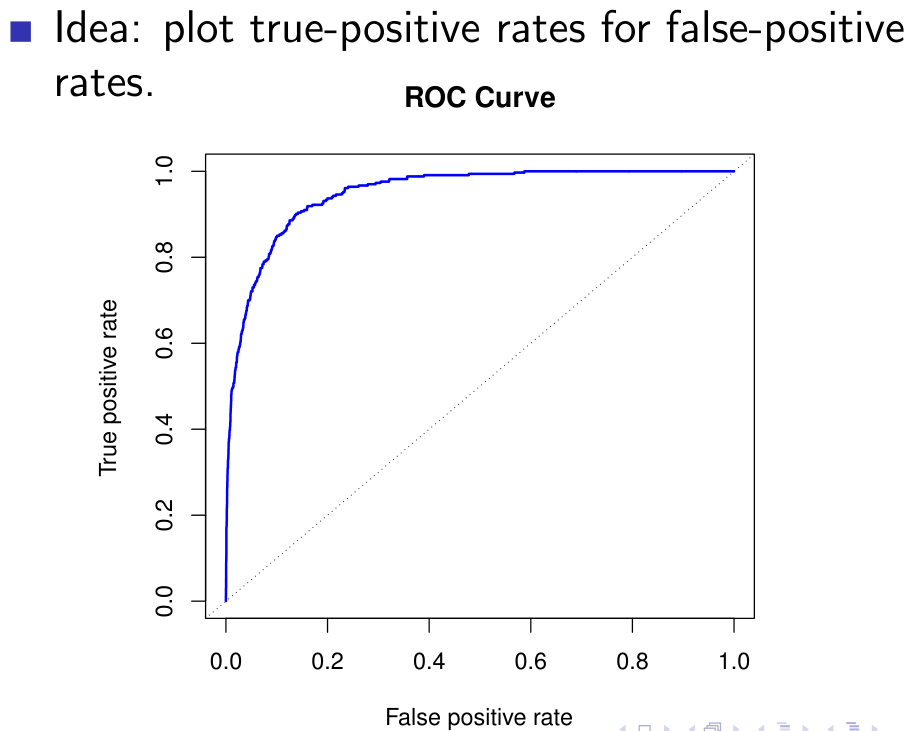
\includegraphics[width=0.7\textwidth]{fig/roc.png}
\caption{Curva ROC.}
\label{fig:roc}
\end{figure}

Podemos selecionar o melhor $\alpha$ como sendo por exemplo o mais próximo de $(0,1)$. Para um dado classificador, podemos computar a área abaixo da curva ROC, \textit{area under the curve} AUC. O melhor AUC é 1. O AUC $1/2$ é muito ruim. Na realidade, o AUC é uma estimativa de $P(h(x') > h(x'') \mid Y' = 1, Y'' = 0)$.

\subsection{Estatística frequentista}

A estimação de máxima verossimilhança é
$$
\hat{\theta} = \arg \max p(x | \theta),
$$
onde $L(\theta) = p(x | \theta)$ é a probabilidade de fazer as observações $x$ dado o parâmetro $\theta$. A partir das observações, nós obtemos uma estimativa para $\theta$ tentando maximizar a probabilidade de obtermos as observações que de fato observamos.

Para variáveis independentes (o caso em que geral trataremos):
$$
L(\theta) = p(x_1, \ldots, x_n | \theta) = \prod_{i=1}^N p(x_i | \theta).
$$
Para variáveis gaussianas $X_1, \ldots, X_n$ i.i.d. que tiveram observações $x_1, \ldots, x_n$, o princípio de máxima verossimilhança nos dá $\hat{\theta} = \frac{1}{N} \sum_i x_i $.

Um intervalo $(1-\alpha)$ de confiança para $\theta$ é o intervalo $[a, b]$ tal que
$$
P(\theta \in [a, b]) \geq 1-\alpha,
$$
para todo $\theta$.

Para pegarmos o $z$ em função da probabilidade dividido por 2, basta olhar a tabela da Figura \ref{fig:z-tabela}. Note que $z$ é apenas uma parametrização, onde a integral de $\mu$ até $\mu + z \sigma$ da gaussiana dá o respectivo valor da tabela. Como um exemplo, caso queiramos o $z = 1.96$, nós olhamos para a linha $1.9$ e coluna $0.06$ e encontramos o valor $0.4750$ que é o meio da probabilidade, ou seja $0.4750 \times 2 = 95\%$ do intervalo de confiança. Para uma distribuição normal, este é $\qty[\mu - \frac{z \sigma}{\sqrt{N}}, \mu + \frac{z \sigma}{\sqrt{N}}]$.
\begin{figure}[H]
\centering
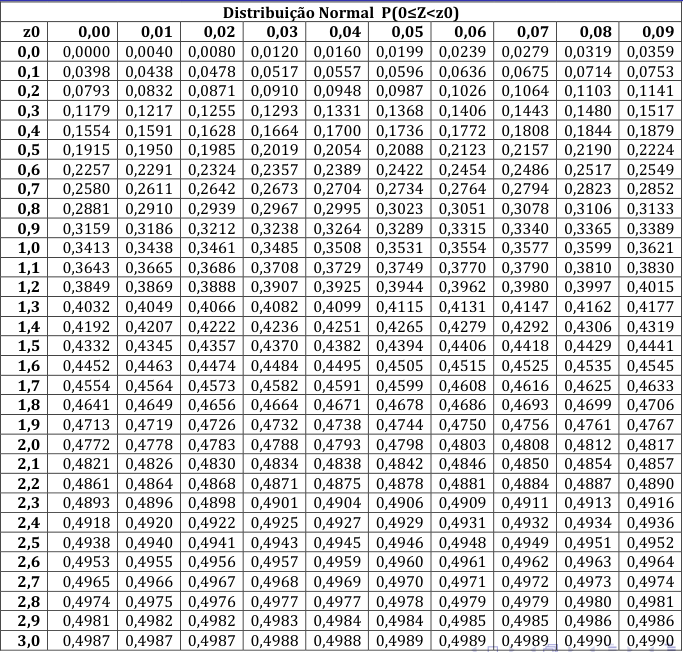
\includegraphics[width=0.5\textwidth]{fig/z-tabela.png}
\caption{Tabela de intervalo de confiança.}
\label{fig:z-tabela}
\end{figure}

Para o erro empírico $\hat{e}_r$ a partir de $M$ observações, ainda sim olhamos a tabela da Figura \ref{fig:z-tabela} para descobrimos a relação entre $z$ e o valor do intervalo de confiança. Então usamos a fórmula
$$
\qty[\hat{e}_r - z \sqrt{\frac{\hat{e}_r(1-\hat{e}_r)}{M}},
\hat{e}_r + z \sqrt{\frac{\hat{e}_r(1-\hat{e}_r)}{M}}],
$$
que indica a taxa de erro de probabilidade $1-\alpha$ que produz o $z$ de acordo com a tabela.

\subsubsection{Teste de hipótese}

Começamos com uma hipótese nula $H_0: \theta \in \Theta_0$ e uma hipótese alternativa $H_1: \theta \in \Theta_1$. Então coletamos dados e checamos se a hipótese nula é rejeitada: rejeitamos-a quando os dados caem dentro de uma região de rejeição $R$. Existem dois tipos de erro nesse processo:
\begin{itemize}
\item Erro tipo I: quando se rejeita $H_0$ e ele é verdadeiro.
\item Erro tipo II: não se rejeita $H_0$ quando ele é falso.
\end{itemize}

 A ideia é escolher uma região de rejeição $R$ que controle o erro tipo I. O nível de $R$ é $\alpha$ quando a probabilidade de erro tipo I é menor ou igual que $\alpha$, dado que $H_0$ é verdadeiro.

Exemplo: $X_i \sim N(\theta, \sigma)$.

Teste:
$$
\begin{cases}
\; H_0: \theta \leq 0, \\
\; H_1: \theta > 0.
\end{cases}
$$
Região de rejeição
$$
R = \qty{x_1, \ldots, x_n: \frac{1}{N} \sum_i x_i > c}.
$$

Escolhemos $c$ de maneira que $P(X \in R \mid \theta) \leq \alpha$ para todo $\theta \in H_0$. Um teste com o menor erro do tipo II para cada $\alpha$ é o \textit{teste mais forte}.

\n

O conceito de $p-$\textit{valor} é o seguinte:
\begin{itemize}
\item Faça um teste: rejeite $H_0$ se, e somente se, $T(x_1, \ldots, x_N) \geq c$.
\item O $p-$valor é
\begin{itemize}
\item o menor nível $\alpha$ em que podemos rejeitar $H_0$.
\item ou a máxima probabilidade de que $T(X_1, \ldots, X_N)$ é maior que $T(x_1, \ldots, x_N)$ quando $H_0$ é verdadeiro.
\end{itemize}
\item um $p-$valor muito pequeno é uma evidência forte contra $H_0$.
\item tipicamente $<0.01$ é muito forte contra $H_0$, já com $>0.1$ tem-se pouca evidência contra $H_0$.
\end{itemize}

\n

Suponha que tenhamos dois classificadores e um dataset de teste. Queremos testar se eles têm taxas de erro iguais. Nós fazemos validação cruzada $k-$fold, e então aplicamos ambos os clasificados em cada fold. Isso nos dá $k$ pares $(a_1, b_1), \ldots, (a_k, b_k)$. Então assumimos que a distribuição de acurácias é Gaussiana com variâncias iguais, mas desconhecidas. A hipótese nula é que não tem diferença.

Wald test com $\alpha$: rejeitar $H_0$ se $\abs{W} > z$, onde $P(-z \leq Z \leq z) = 1-\alpha$ e
$$
W = \frac{\mu}{s},
$$
onde $\mu = \sum_{i=1}^N (a_i - b_i)/N$ e
$$
s = \sqrt{\frac{1}{N(N-1)}\sum_{i=1}^N \qty(a_i-b_i-\frac{1}{N}\sum_{j=1}^N (a_j-b_j))^2}.
$$
Como $W$ é assintoticamente gaussiano, temos o intervalo de confiança para a diferença entre os dois classificadores $\qty[\mu - zs, \mu + zs]$, onde $z$ é relacionado a $1-\alpha$ pela Figura \ref{fig:z-tabela}.

\section{Regression}

Lembre que temos o modelo $Y = f(X) + \eps$, onde $\eps$ é independente de $f$ e tem média zero. Regressão linear adota $f(X) = \beta_0 + \beta_1 X_1 + \cdots + \beta_n X_n$.

O método de mínimos quadrados é:
\begin{itemize}
\item Suponha que tenhamos as observações $x_{1j}, x_{2j}, \ldots, x_{nj}, y_j$, para $j \in \{1, \ldots, N\}$.
\item Consideremos o \textit{residual sum of squares} que tentaremos minimizar pelos parâmetros $\beta_0, \beta_1, \ldots, \beta_n$.
$$
\text{RSS} = \sum_{j=1}^N (y_j - f(x_j))^2.
$$

\subsection{Regressão Linear Simples}

Nós temos $Y = \beta_0 + \beta_1 X_1$. Para minimizar RSS:
$$
\hat{\beta}_0 = \cc{y} - \hat{\beta}_1 \cc{x}_1,
$$
$$
\hat{\beta}_1 = \frac{\sum_j (x_{1j} - \cc{x}_1) (y_j - \cc{y})}{\sum_j (x_{1j}-\cc{x}_1)^2},
$$
onde $\cc{x}_1 = \frac{1}{N} \sum_{j=1}^N x_{1j}$ e $\cc{y} = \frac{1}{N} \sum_{j=1}^N y_j$.

A estimativa $\hat{\sigma}^2$ \textit{unbiased} para $\sigma^2$ deve levar em conta os dois graus de liberdade. Logo
$$
\hat{\sigma}^2 = \frac{1}{N-2} \sum_{j=1}^N (y_j - \hat{y}_j)^2.
$$
Existe um teste padrão para $H_0: \beta_1 = 0$ versus $H_1: \beta_1 \neq 0$. Rejeite $H_0$ quando
$$
\abs{\frac{\hat{\beta}_1}{\sqrt{\hat{\sigma}^2 \sum_{j=1}^N (x_{1j}-\cc{x}_1)^2}}}>z.
$$
\end{itemize}

O $p-$valor para esse caso funciona assim. Faça um teste da forma $T > c$ para $T$ que dependa dos dados, e algum $c$. Então um $p-$valor é a probabilidade que $T$ seja maior que o $T$ observado, para $H_0$ verdadeiro (ou seja, $\beta_1 = 0$). Lembrando que $p-$valor pequeno é uma evidência contra $H_0$.

Uma medida comum do fit é o $R^2$. No caso geral $X_1, X_2, \ldots, X_n$:
$$
R^2 = 1 - \frac{\text{RSS}}{\sum_{j=1}^N (y_j - \cc{y})^2},
$$
que é a proporção da variabilidade do $Y$ que pode ser explicada por $X_1, \ldots, X_n$. $R^2$ está entre 0 e 1. Quando maior melhor.

No caso de uma variável $X_1$ somente, temos a expressão
$$
R^2 = \qty(\frac{\sum_{j=1}^N (x_{1j}-\cc{x}_1)(y_j-\cc{y})}
{\sqrt{\sum_{j=1}^N (x_{1j}-\cc{x}_1)^2}\sqrt{\sum_{j=1}^N (y_j-\cc{y})^2}})^2 =
\qty(\frac{E[(X_1-E(X_1))(Y-E(Y))]}{\sigma_{X_1} \, \sigma_Y})^2 =
$$
$$
= \frac{\text{cov}(X_1, Y)^2}{\sigma_{X_1}^2 \sigma_Y^2} =
\rho_{X_1, Y}^2.
$$
Note que isso é a correlação entre $X_1$ e $Y$.

\subsection{Caso mais geral}

Para muitas variáveis $Y = \beta_1 X_1 + \cdots + \beta_n X_n + Z$ (note que $\beta_0 = 0$), com $E[Z] = 0$, o RSS é $(C-AB)^T (C-AB)$, onde
$$
A =
\begin{pmatrix}
x_{11} & x_{12} & \cdots & x_{n1} \\
\vdots & \vdots & \ddots & \vdots \\
x_{1N} & x_{2N} & \cdots & x_{nN} \\
\end{pmatrix}, \quad
B =
\begin{pmatrix}
\beta_1 \\
\vdots \\
\beta_n \\
\end{pmatrix}, \quad
C =
\begin{pmatrix}
y_1 \\
\vdots \\
y_n \\
\end{pmatrix},
$$
e os $\beta_i$ que minimizam o RSS são
$$
\hat{B} = (A^T A)^{-1} A^T C.
$$
Se $Z$ tem variância $\sigma^2$, então $\hat{B}$ tem variância $\sigma^2 (A^T A)^{-1}$ e é aproximadamente gaussiano para grande $N$.

Novamente, podemos testar a variabilidade do $Y$ com $X_1, X_2, \ldots, X_n$ através do
$$
R^2 = 1 - \frac{\text{RSS}}{\sum_{j=1}^N (y_j - \cc{y})^2}.
$$

\subsection{Covariate selection}

Geralmente, devemos descartar algumas covariáveis. Assim, devemos dar um \textit{score} para cada conjunto de variáveis, e escolher o melhor. Um score popular é o AIC (Akaike Information Criterion):
$$
L_S - \abs{S}, \text{ (goodness of fit} - \text{model complexity),}
$$
onde $S$ é o conjunto de covariáveis no modelo scored e $L_S$ é a log-likelihood do modelo com covariáveis em $S$, avaliada na estimação de máxima verossimilhança.

Outro popular é o BIC (Bayesian Information Criterion):
$$
L_S - \frac{\abs{S}}{2} \log N.
$$
Para $N$ grande, a probabilidade posterior do scored model é proporcional a $e^{\text{BIC}}$, quando todos os modelos têm probabilidade idêntica.

Outro score é o \textit{Mallow's} $C_p$:
$$
2 \abs{S} \hat{\sigma}^2 + \sum_{j=1}^N (\hat{y}_j^S - y_j)^2,
$$
onde $\hat{\sigma}^2$ é a estimativa da unbiased variância com todas as covariáveis, enquanto $\hat{y}_j^S$ são produzidos com covariáveis somente em $S$. Esse score estima o erro de treino que é esperado de um modelo com covariáveis em $S$.

Structure search:
\begin{itemize}
\item Forward stepwise regression: começar sem covariáveis, adicionar uma que leva ao melhor score, depois adicionar outra que leva ao melhor score, etc.
\item Backward stepwise regression: começar com todas as covariáveis, retirar aquela que leva ao melhor score, etc.
\end{itemize}

Quando se tem features qualitativas:
\begin{itemize}
\item Fazer algum encoding (transformar em números, ou outros data structures).
\item Se os valores forem ordenados: transformá-los em números.
\item Se não for apropriado ordená-los: \textit{one-hot} encoding. Ou seja, para cada valor único numa coluna qualitativa, uma nova coluna é criada. Então essas novas variáveis são preenchidas com zeros e uns (1 significando \texttt{True} e 0 \texttt{False}).
\end{itemize}

Nonlinear terms in regression: colocar termos que não são lineares, LOL.

Polynomial regression: quando as funções são polinômios das covariáveis.

\subsection{Regularização}

A ideia é penalizar o ``tamanho'' dos parâmetros, para reduzir a variância (mas com um aumento no bias). Isso é útil para reduzir overfitting. As duas principais estratégias são \textit{ridge regression} e \textit{lasso}.

\n

No Ridge a gente só adiciona um novo termo $\lambda \sum_{i=1}^N \beta_i^2$. Agora minimazeremos
$$
\sum_{j=1}^N \qty(y_j - \sum_{i=1}^n \beta_i x_{ij})^2 + \lambda \sum_{i=1}^n \beta_i^2.
$$
Quanto maior o parâmetro $\lambda \geq 0$ menor os valores de $\hat{\beta}_i$. Para tunar $\lambda$ geralmente se faz cross-validation.

A solução é fácil (mas biased):
$$
\hat{B} = (A^TA + \lambda I)^{-1} A^T C.
$$

Em regressão linear, multiplicar as covariáveis leva à estimativas multiplicadas. Assim, uma suposição usual é que os dados estejam normalizados (média 0 e variância 1):
$$
\tilde{x}_{ij} = \frac{x_{ij}}{\sqrt{\frac{1}{N}\sum_{j=1}^N (x_{ij} - \cc{x}_{i})^2}},
$$
e que $Y$ é centrado (a média é subtraída).

\n

Na regressão Lasso nós minimizamos
$$
\sum_{j=1}^N \qty(y_j - \sum_{i=1}^n \beta_i x_{ij})^2 + \lambda \sum_{i=1}^n \abs{\beta_i},
$$
e novamente tunamos $\lambda$ com cross-validation, normalizamos $X_i$ e centralizamos $Y$.

Amazing fact: se $\lambda$ é grande o bastante, muitos dos $\beta_i$ são setados à zero. Logo, feature selection é feita automaticamente.

Com o lasso, não existe solução analítica fechada. Mas dá para fazer a minimazação com otimização convexa.

Tanto Ridge quanto Lasso minimizam RSS, mas
\begin{itemize}
\item Ridge: sujeito a $\sum_i \beta_i^2 \leq \tilde{\lambda}$.
\item Lasso: sujeito a $\sum_i \abs{\beta_i} \leq \tilde{\lambda}$.
\end{itemize}
\begin{figure}[H]
\centering
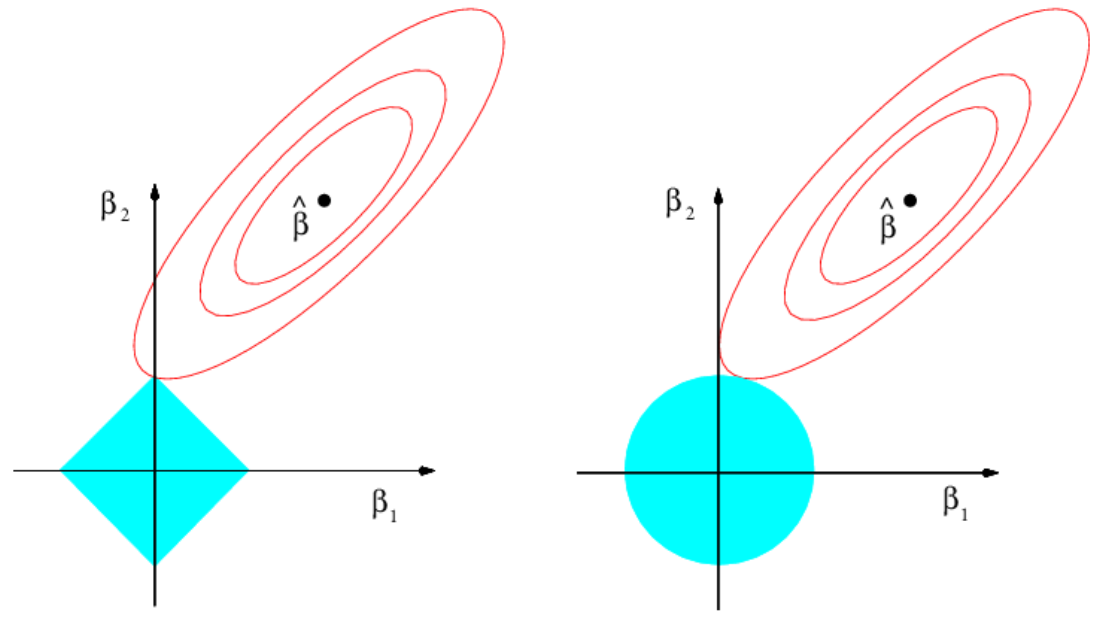
\includegraphics[width=0.5\textwidth]{fig/ridge-lasso.png}
\caption{Ridge vs Lasso.}
\label{fig:ridge-lasso}
\end{figure}

\section{Logistic regression}

Suponha que $Y$ seja binário (valores 0 ou 1, problema de classificação). Nós assumimos que
$$
P(Y=1 \mid X_1, \ldots, X_n) = \frac{e^W}{1 + e^W},
$$
onde
$$
W = \sum_{i=1}^n \beta_i X_i.
$$

Equivalentemente
$$
\text{logit}(P(Y=1 \mid X_1, \ldots, X_n)) = \sum_{i=1}^n \beta_i X_i,
$$
onde $\text{logit}(p) = \log(p/(1-p))$.

A fronteira
$$
\frac{e^W}{1+e^W} = 1/2
$$
é dada pela equação linear $W = \sum_{i=1}^n \beta_i X_i = 0$.

A likelihood function dadas observações $x_{ij}, y_j$ é
$$
L(\beta_1, \ldots, \beta_n) =
\prod_{j=1}^N \qty(\frac{e^{\sum_{i=1}^N \beta_i x_{ij}}}{1 + e^{\sum_{i=1}^N \beta_i x_{ij}}})^{y_j} \qty(1 - \frac{e^{\sum_{i=1}^N \beta_i x_{ij}}}{1 + e^{\sum_{i=1}^N \beta_i x_{ij}}})^{1-y_j}.
$$

Problema: não existe solução fechada para o máximo da função de likelihood acima. Um algoritmo popular para resolver a maximização acima é o IRLS (Iterative Reweighted Least Squares Algorithm).

\subsection{IRLS}

\begin{enumerate}
\item Comece com um chute $\hat{\beta}_i^0$.
\item Repita até a convergência:
\begin{enumerate}
\item $p_j \leftarrow \frac{e^{\sum_{i=1}^N \beta_i x_{ij}}}{1+e^{\sum_{i=1}^N \beta_i x_{ij}}}$.
\item $q_j \leftarrow \text{logit}(p_j) + \frac{y_j - p_j}{p_j(1-p_j)}$.
\item $F \leftarrow \text{diag}\Big(p_1(1-p_1), p_2(1-p_2), \ldots, p_N(1-p_N)\Big)$.
\item Coloque
$$
\begin{pmatrix}
\hat{\beta}_1 \\
\vdots \\
\hat{\beta}_n \\
\end{pmatrix} \leftarrow
(A^T FA)^{-1} A^T F
\begin{pmatrix}
q_1 \\
\vdots \\
q_N \\
\end{pmatrix}.
$$
\end{enumerate}
\end{enumerate}

\subsection{LDA}
Suponha que tenhamos uma classe binária e uma feature contínua, e
\begin{itemize}
\item $X$ dado $Y = 0$ é gaussiana $\s{N}(\mu_0, \sigma^2)$.
\item $X$ dado $Y = 1$ é gaussiana $\s{N}(\mu_1, \sigma^2)$.
\end{itemize}
Para obter $P(Y = 1 \mid x)$, utilizar a regra de Bayes
$$
P(Y = 1 \mid x) =
\frac{p(x \mid Y=1) P(Y=1)}{\sum_k p(x \mid Y=k) P(Y=k)}.
$$
Então o classificador de Bayes é
$$
\begin{cases}
\; 1 \; \text{ se } \log(\frac{P(Y=1)}{P(Y=0)}) - r_1^2 + r_0^2 > 0 \\
\; 0 \; \text{ caso contrário,}
\end{cases}
$$
$$
\iff
\begin{cases}
\; 1 \; \text{ se } 2x(\mu_1-\mu_0) > \mu_1^2 - \mu_0^2 - 2\sigma^2 \log(\frac{P(Y=1)}{P(Y=0)}) \\
\; 0 \; \text{ caso contrário,}
\end{cases}
$$
onde $r_i^2 = (x-\mu_i)^2/2\sigma^2$. Note que a expressão acima é linear.

\subsection{QDA}

Mesmas hipótese que no LDA, mas agora $X$ dado $Y=0$ ou $Y=1$ tem variâncias diferentes $\sigma_0^2$ e $\sigma_1^2$. O classificador Bayes é
$$
\begin{cases}
\; 1 \; \text{ se } r_1^2 - r_0^2 < \log(\frac{\sigma_0 P(Y=1)}{\sigma_1 P(Y=0)}) \\
\; 0 \; \text{ caso contrário.}
\end{cases}
$$

Então o QDA é: use o classificador plug-in de máxima verossimilhança.

\subsection{Comparação}

\begin{itemize}
\item Para o LDA, com dois labels, a fronteira de classificação é uma função linear dos features.
\item Assim, o LDA tem o mesmo comportamento que a regressão logística.
\begin{itemize}
\item Mas o LDA é construído estimando as probabilidades de $Y$ e das features, enquanto que a regressão logística foca em estimar os coeficientes de fronteira.
\item Regressão logística é geralmente melhor que LDA.
\end{itemize}
\end{itemize}

Observações:
\begin{itemize}
\item LDA, Naive Bayes etc, são \textit{generativos}: eles tentam modelar $P(X, Y)$.
\item Regressão logística é \textit{discriminativo}: ela teta modelar $P(Y \mid X)$.
\item A primeira é mais ``perto da verdade'' ??, mas a última é geralmente mais exata.
\end{itemize}


\section{SVM}

Consideremos um problema classificação binário com $Y \in \{-1, 1\}$.

Suponha que as classes ($Y$) são separáveis linearmente por um hiperplano
$$
H(X) = \beta_0 + \beta_1 X_1 + \cdots + \beta_n X_n = 0,
$$
ou seja, temos esse tipo de situação
\begin{figure}[H]
\centering
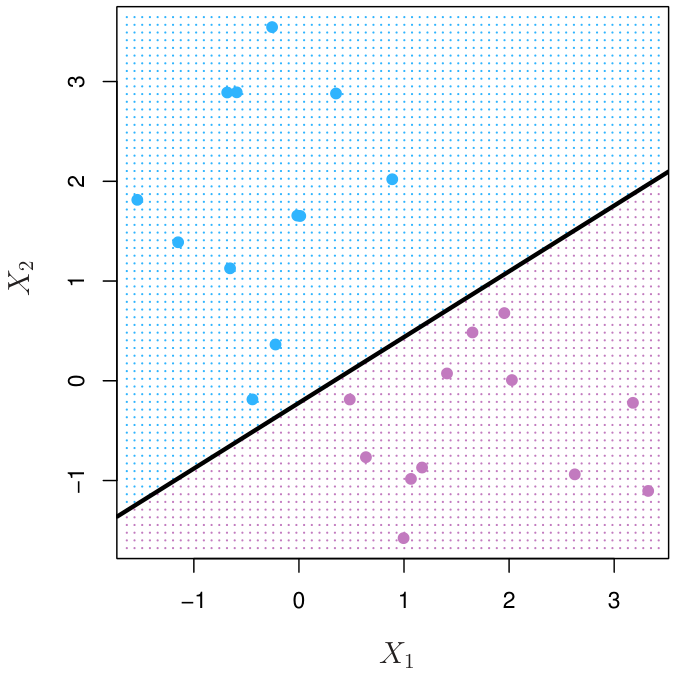
\includegraphics[width=0.5\textwidth]{fig/linear-separable.png}
\caption{Separação linear das classes.}
\label{fig:linear-separable}
\end{figure}

Quando existirem vários hiperplanos possíveis que separam os dados, pegue o hiperplano com margem máxima. A margem é a distância do hiperplano para o ponto de treino mais próximo.
\begin{figure}[H]
\centering
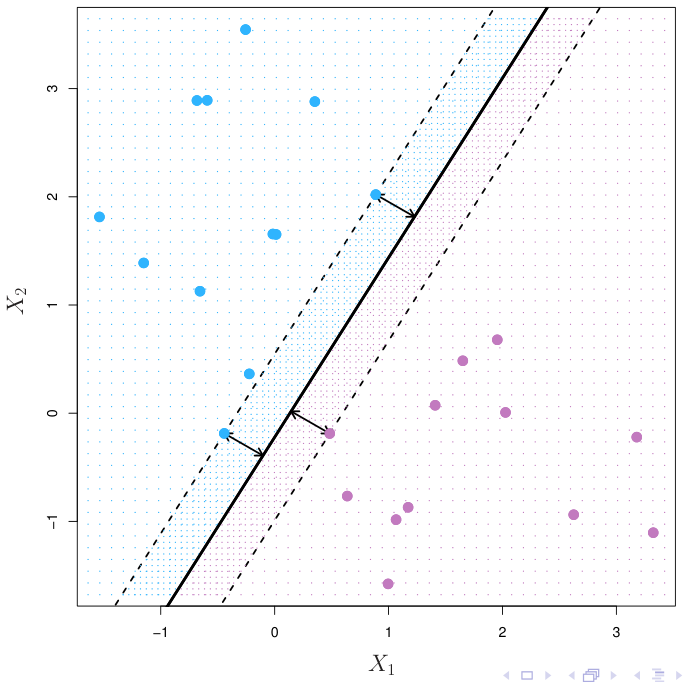
\includegraphics[width=0.5\textwidth]{fig/max-margin.png}
\caption{Escolha do plano com maior margem.}
\label{fig:max-margin}
\end{figure}

Para o hiperplano com margem maximal, os vetores suportes são os pontos que estão mais próximos dele. Para tal hiperplano, a distância da observação $i$ até o hiperplano é dada por
$$
\frac{y_j(\beta_0 + \beta_1 x_{1j} + \cdots + \beta_n x_{nj})}{\sqrt{\beta_1^2 + \cdots + \beta_n^2}}.
$$

Então tente achar $\beta_0, \beta_1, \ldots, \beta_n$ que maximize $M$ tal que
$$
\sum_{i=1}^n \beta_i^2 = 1 \e
y_j(\beta_0 + \beta_1 x_{1j} + \cdots + \beta_n x_{nj}) \geq M, \ptodo j.
$$

Esse tipo de problemas de otimização pode ser resolvido rapidamente utilizando programação quadrática. O mínimo é garantido de ser achado.

Na prática, claramente os problemas são não-separáveis. Se um problema é não-separável, então não há solução com $M > 0$. O problema então deve ser relaxado. Considere uma \textit{softmargin}: deixemos algumas observação violar a margem. Daí a situação fica com margens soft pontilhadas:
\begin{figure}[H]
\centering
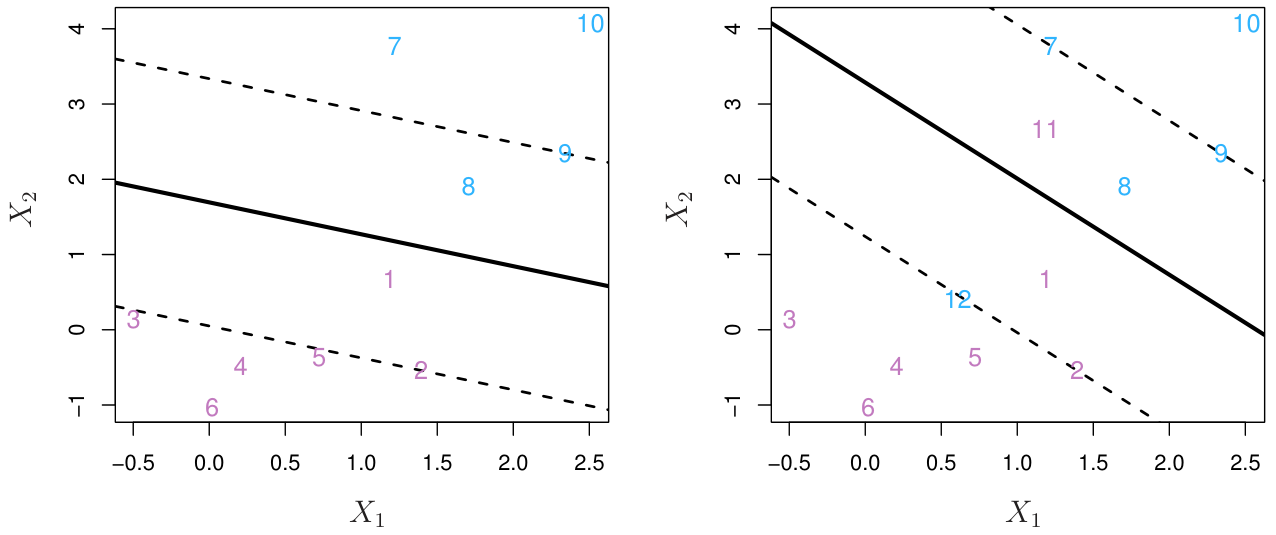
\includegraphics[width=0.5\textwidth]{fig/soft-margin.png}
\caption{Margem soft em pontilhado.}
\label{fig:soft-margin}
\end{figure}

O problema de otimização \textit{soft} é então achar $\beta_0, \beta_1, \ldots, \beta_n$ e $\eps_1, \ldots, \eps_N$ que maximizam $M$ sujeitos a
$$
\sum_{i=1}^n \beta_i^2 = 1 \e
y_j(\beta_0 + \beta_1 x_{1j} + \cdots + \beta_n x_{nj}) \geq M (1-\eps_j),
$$
para cada $j$ e
$$
\eps_j \geq 0, \quad \sum_{j=1}^N \eps_j \leq C.
$$

Alguns pontos:
\begin{itemize}
\item O problema soft pode ser resolvido por programação quadrática.
\item Importante: apenas observações dentro da margem afetam o hiperplano.
\begin{itemize}
\item Apenas as fronteiras importam.
\item SVMs estão mais próximas de classificadores discriminativos do que generativos.
\end{itemize}
\item O hiperparâmetro $C$ é geralmente tunado por cross-validation.
\begin{itemize}
\item Se $C$ é zero, não relaxação; Quanto maior $C$, mais pontos de treino podem estar dentro da margem.
\end{itemize}
\end{itemize}

\section{Nonlinear boundaries}

Podemos capturar fronteiras não lineares engrandecendo as features, por exemplo
$$
X_1, X_1^2, X_2, X_2^2, \ldots, X_n, X_n^2,
$$
e talvez outras funções de features.

A estrutura das SVMs permitem fazer isso eficientemente para espaços muito engrandecidos, usando os \textit{kernels}.

Acontece que SVMs podem ser aprendidas apenas tratando dos produtos internos $x' \vdot x''$, onde $x'$ e $x''$ são duas observações. Suponha que tenhamos funções $\phi(X) = [\phi_1(X), \ldots, \phi_m(X)]$, então precisaríamos das quantidades $\phi(x') \vdot \phi(x'')$. Ao invés disso, podemos apenas utilizar a função $K(X', X'')$ toda vez que um produto escalar é necessário. Tal função é chamada \textit{kernel}.

\n

Popular kernels:
\begin{itemize}
\item Polinomial: $K(X', X'') = (1 + X' \vdot X'')^d$.
\item Base radial: $K(X', X'') = \exp(-\gamma\norm{X' \vdot X''})$.
\item Neural: $K(X', X'') = \tanh(\gamma_1(X' \vdot X'') + \gamma_2)$.
\end{itemize}

Os hiperparâmetros dos kernels são, como sempre, tunados por cross-validation.
\begin{figure}[H]
\centering
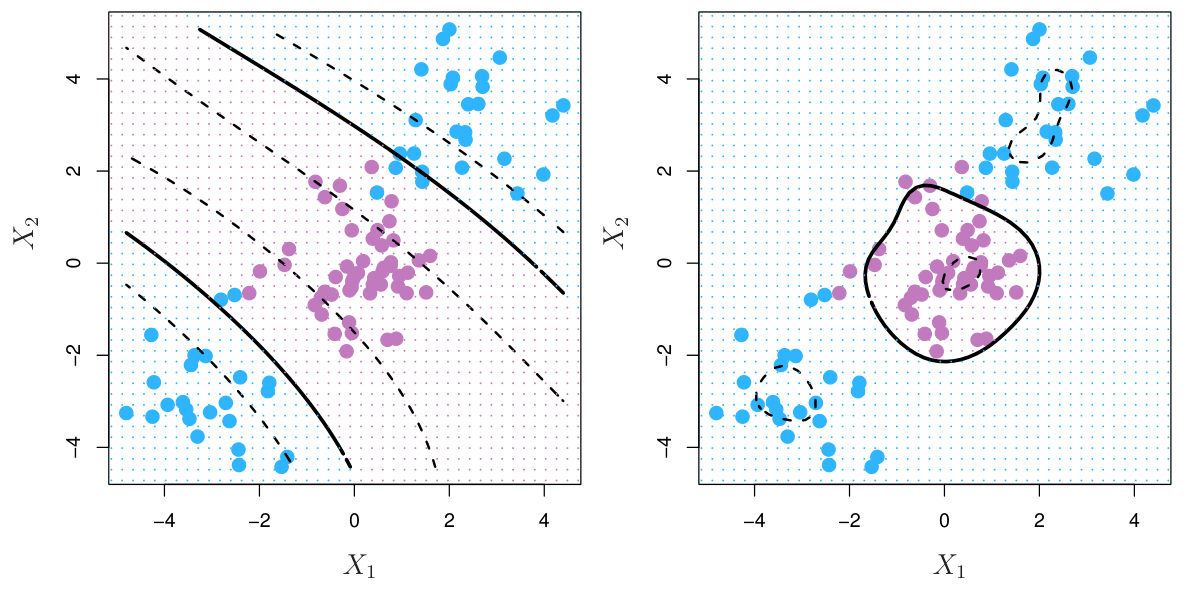
\includegraphics[width=0.5\textwidth]{fig/kernel.png}
\caption{SVM quando kernels são aplicados.}
\label{fig:kernel}
\end{figure}


\end{document}
